\documentclass[10pt,a4paper]{article} 
\fontfamily{cmss}
\usepackage{amsmath}
\usepackage{bm}
\usepackage{amssymb}
\usepackage{mathtools}
\usepackage[brazilian]{babel}
\usepackage[utf8]{inputenc}
\usepackage[T1]{fontenc}
\usepackage[parfill]{parskip}
\usepackage[margin=1.0in]{geometry}
\usepackage{graphicx}
\usepackage{type1ec}
\usepackage{graphicx}
\usepackage{listings}

\begin{document}

	% CABECALHO %

	\begin{minipage}[b]{0.05\linewidth}
		%\begin{figure}
			
\includegraphics[scale=0.3]{ufmg}
		%\end{figure}
	\end{minipage}
	\hfill
	\begin{minipage}[b]{0.95\linewidth}
		\begin{flushright}
			\textbf{UNIVERSIDADE FEDERAL DE MINAS GERAIS} \\
			\textsc{Graduação em Engenharia de Sistemas} \\
			\textbf{Otimização Não Linear - Trabalho Computacional 2} \\
			2017-02 \\
			Prof. Felipe Campelo \\
			Matheus Silva Araujo - 2013066265
		\end{flushright}
	\end{minipage}

	\begin{center}
		\hrulefill
	\end{center}

	% CABECALHO %

	\section{Introdução}

	O segundo Trabalho Computacional da disciplina Otimização Não Linear tem como objetivo avaliar métodos de otimização de problemas restritos.

	Para isso serão implementados e avaliados dois métodos:

	\begin{itemize}

		\item Método das Penalidades Exteriores

		\item Método das Penalidades Interiores

	\end{itemize}

	Métodos de Penalidades transformam o problema restrito em um problema irrestrito equivalente através de funções de penalidades.

	\section{Método de Penalidades Exteriores}

	\subsection{Conceito}

	O método de \emph{Penalidades Exteriores}, ou \emph{Penalidades Externas}, converte o problema restrito em um problema irrestrito criando uma função de penalidade, $P(\bm{x})$, definida por:

	$$ P(\bm{x}) = r^h \sum_{j=1}^{m} h_j (\bm{x})^2 + r^g \sum_{u=1}^l(\text{max}(0,g_i(\bm{x})))^2 $$

	O algoritmo soma a função $P(\bm{x})$ à função objetivo e otimiza essa função resultante. Ele repete o processo alterando os fatores de penalidade $r^h$ e $r^g$ até que $P(\bm{x}) = 0$.

	A função $P(\bm{x})$ \emph{penaliza} violações das restrições e aproxima da solução ótima \emph{externamente}. 

	\subsection{Avaliação}

	O método de Penalidades Exteriores foi avaliado na otimização da seguinte equação:

	$$ \bm{x^*} = \underset{\bm{x}}{\text{arg min}} f(\bm{x}) = x_1^4 - 2x_1^2x_2 + x_1^2 + x_1x_2^2 - 2x_1 + 4$$

	Sujeita a:

	$$ g_1(\bm{x}) = 0.25x_1^2 + 0.75x_2^2-1 \le 0 $$ 
	$$ h_1(\bm{x}) = x_1^2+x_2^2-2=0 $$

	\subsection{Resultados}

	\begin{figure}[h]
		\centering
		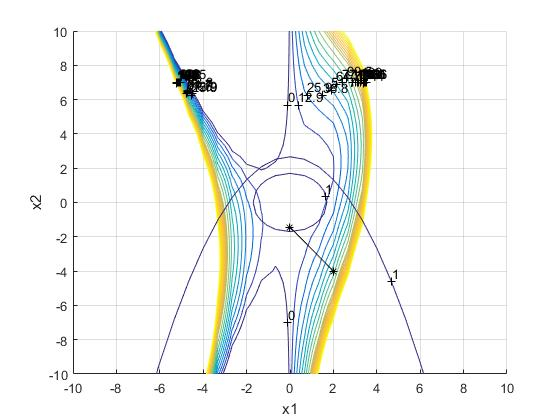
\includegraphics[width=11cm]{penalidade_exterior}
		\caption{Método de Penalidades Exteriores}
		\label{penalidade_exterior}
	\end{figure}

	A trajetória dos pontos obtidos durante a otimização utilizando o método de \emph{Penalidades Exteriores} é mostrado na Figura \ref{penalidade_exterior}.

	Os valores finais encontrados foram:

	\begin{itemize}

		\item Ponto final: $\bm{x} = [-0.006157 -1.430599]$
		\item Valor da função objetivo no ponto: $f(\bm{x}) = 3.99986$
		\item $r^h = r^g = 0.500000$

	\end{itemize}

	\section{Método de Penalidades Interiores}

	\subsection{Conceito}

	O método de \emph{Penalidades Interiores}, ou \emph{Método de Barreira}, converte o problema restrito em um problema irrestrito criando uma função de barreira, $b(\bm{x})$, definida por:

	$$b(\bm{x}) = -u \sum_{i=1}^l \frac{1}{g_i(\bm{x})}$$

	O algoritmo soma a função $b(\bm{x})$ à função objetivo e otimiza essa função resultante. Ele repete o processo alterando o fator de penalidade $u$ até que um critério de parada desejado seja atingido.

	Funções de barreira não podem ser definidas para restrições de igualdade.

	A função $b(\bm{x})$ \emph{penaliza saídas} da região factível e aproxima da solução ótima \emph{internamente}. 

	\subsection{Avaliação}

	O método de Penalidades Interiores foi avaliado na otimização da seguinte equação:

	$$ \bm{x^*} = \underset{\bm{x}}{\text{arg min}} f(\bm{x}) = (x_1-5)^2+(x_2-3)^2$$

	Sujeita a:

	$$ g_1(\bm{x}) = x_1 + x_2 -3 \le 0 $$ 
	$$ g_2(\bm{x}) = -x_1 + 2x_2 - 4 \le 0 $$ 

	\subsection{Resultados}

	\begin{figure}[h]
		\centering
		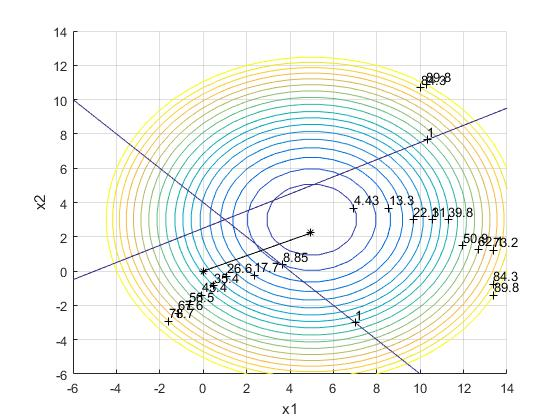
\includegraphics[width=11cm]{penalidade_interior}
		\caption{Método de Penalidades Interiores}
		\label{penalidade_interior}
	\end{figure}

	A trajetória dos pontos obtidos durante a otimização utilizando o método de \emph{Penalidades Interiores} é mostrado na Figura \ref{penalidade_interior}.

	Os valores finais encontrados foram:

	Os valores finais encontrados foram:

	\begin{itemize}

		\item Ponto final: $\bm{x} = [4.963174 2.224315]$
		\item Valor da função objetivo no ponto: $f(\bm{x}) = 0.603044$
		\item $r^h = r^g = 5.000000$

	\end{itemize}

	\section{Conclusão}

	Através do segundo Trabalho Computacional da disciplina Otimização Não Linear foi possível avaliar o funcionamento dos métodos de penalidades 
	externa e interna.

	Nos dois métodos foram necessárias poucas iterações para encontrar o ponto de ótimo. No método de \emph{Penalidade Interior}, o mínimo encontrato estava próximo de $0$.

\end{document}
